
% Homework template for MA 614, Spring 2011.  When a line begins with the percent sign, the typesetter ignores it.  So, use percent signs at the beginning of lines to insert comments to yourself.


% Set the document class.  The command [11pt] sets the font at 11 point, which is nicer to read.  The default would be 10pt
\documentclass[11pt]{amsart} 


% Call packages that allow you to invoke certain mathematical symbols.
\usepackage{amssymb,amsmath,amsthm}
\usepackage[framed,numbered,autolinebreaks,useliterate]{mcode}
\usepackage{graphicx}   % need for figures
% Set the title, author, and date information.
\title{Homework 4}
\author{Anil Aksu}
\date{\today}


% Formally begin the document and make the title.
\begin{document}
\maketitle

\section*{Problem 1 }
Prove relationship : 
\begin{equation*}
\tan \frac{\theta}{2}=\frac{Z e^2 }{4 \pi \epsilon_0 m v^2 b}.
\end{equation*}
for the deflection of an electron of mass $m$ in a Coulomb collision with a much heavier ion, charge Ze. For $\theta /2 $ find the impact parameter $b_0$ and scattering cross-section $\sigma$.
\begin{figure}[h!]
\label{fig:1}
\centering
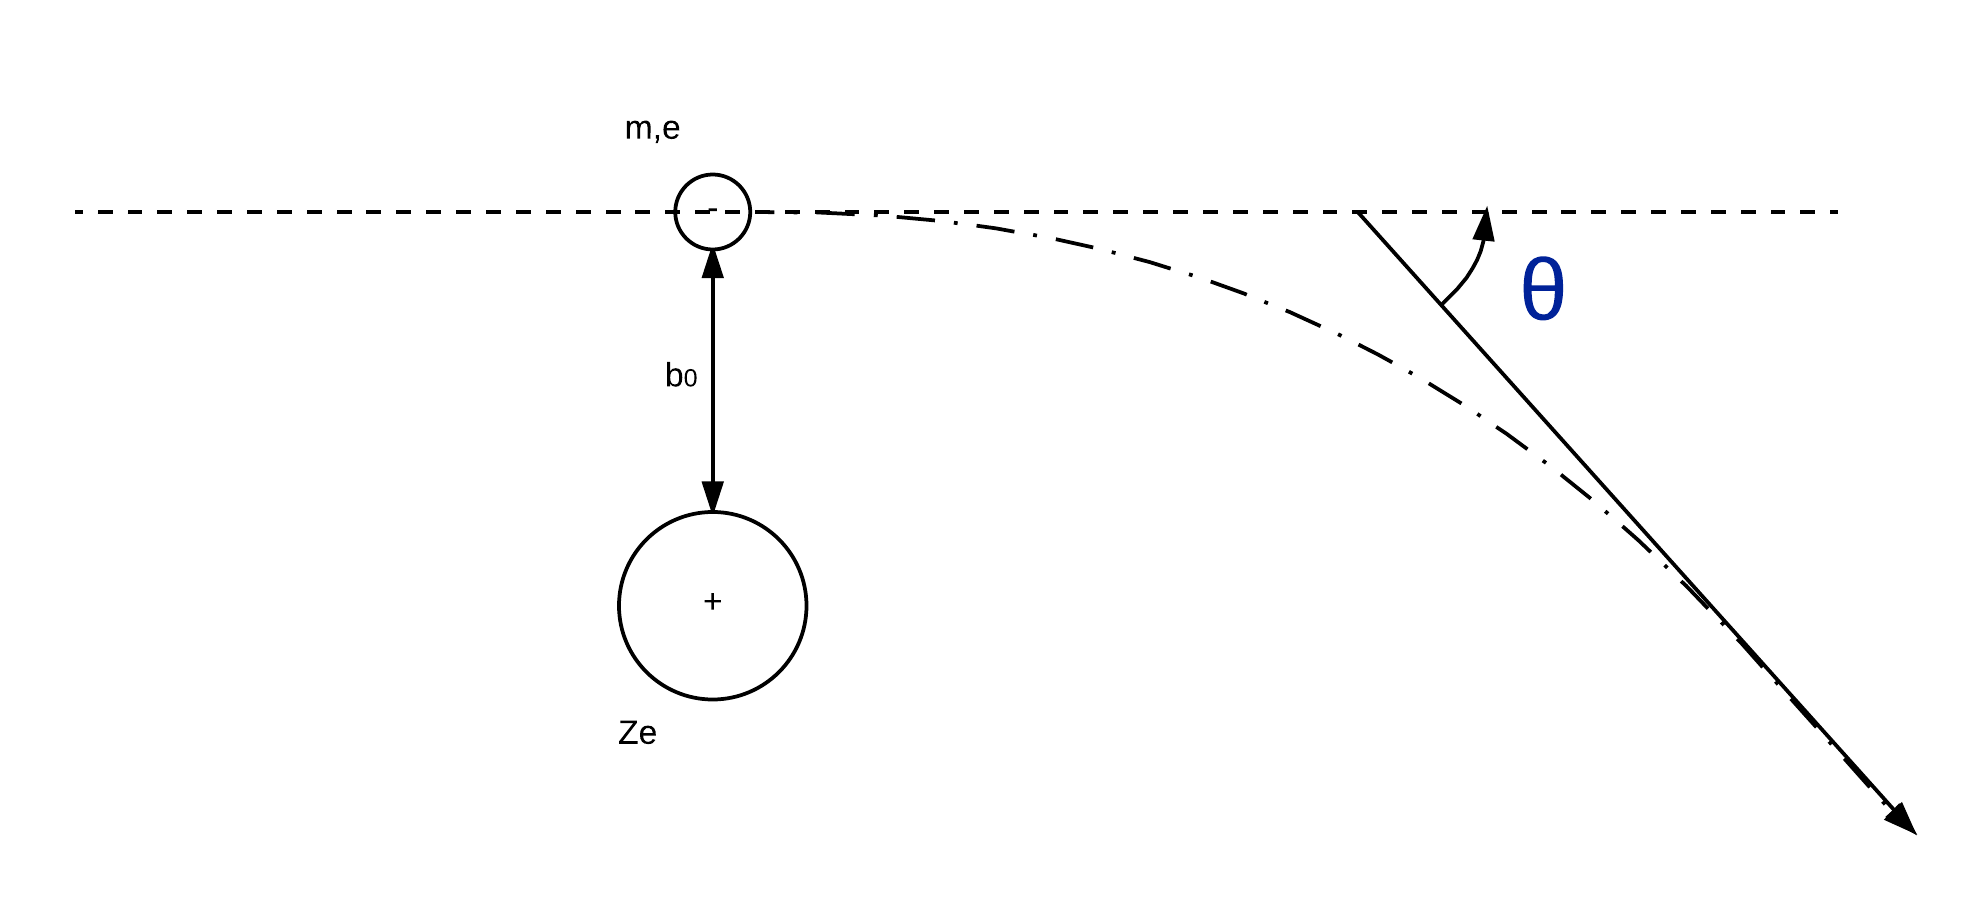
\includegraphics[width = 5in]{ElectronDeviation.png}
\caption{Electron scattering in a Coulomb collision with a much heavier ion. }
\end{figure}
\\
\textbf{Solution:}\\
The equation of motion under electric field generated by a heavier ion in polar coordinates can be given as:
\begin{equation}
\label{eq:1}
m(\ddot{r}-\dot{\alpha}^2 r)=-\frac{Ze^2}{4 \pi \epsilon_0 r^2},
\end{equation}
where $\alpha$ is the radial angle and $r$ is the distance between ion and electron. Equation \ref{eq:1} is the equation of motion in radial direction, however it is not sufficient. Equation of motion in radial direction can be given as:
\begin{equation}
\label{eq:2}
2\dot{r}\dot{\alpha}+r\ddot{\alpha}=0.
\end{equation}
The solution to equation \ref{eq:2} allows us to relate $r$ with $\dot{\alpha}$ as follows:
\begin{equation}
\label{eq:3}
\frac{\ddot{\alpha}}{\dot{\alpha}}=-2\frac{\dot{r}}{r}.
\end{equation}
As a result,
\begin{equation}
\dot{\alpha}=\dot{\alpha}_0 \frac{r_{0}^2}{r^2}.
\end{equation}
Let's define a new variable $\eta = 1/r$ to manipulate equations much easier. Therefore the angular velocity can be written in terms of new variable $\eta$ as:
\begin{equation}
\label{eq:4}
\dot{\alpha}=\dot{\alpha}_0 r_{0}^2 \eta^2.
\end{equation}
Under this formulation, the radius $r$ can be written as a function of $\alpha$. Thus the time derivative with respect to time can be re-expressed as:
\begin{equation}
\label{eq:5}
\dot{r}=\frac{\mathrm{d}}{\mathrm{d}t}\frac{1}{\eta}=-\frac{1}{\eta^2}\frac{\mathrm{d} \eta}{\mathrm{d} \alpha}\dot{\alpha}=-\dot{\alpha}_0 r_{0}^2 \frac{\mathrm{d} \eta}{\mathrm{d} \alpha}.
\end{equation}
And also the second time derivative can be written as:
\begin{equation}
\label{eq:6}
\ddot{r}=-(\dot{\alpha}_0 r_{0}^2)^2 \eta^2\frac{\mathrm{d}^2 \eta}{\mathrm{d} \alpha^2}.
\end{equation}
If the relations in equations \ref{eq:6} and \ref{eq:4} are replaced back into equation \ref{eq:1}, the equation  of motion in radial direction can be re-expressed as:
\begin{equation}
\label{eq:7}
-m(\dot{\alpha}_0 r_{0}^2)^2 \eta^2\frac{\mathrm{d}^2 \eta}{\mathrm{d} \alpha^2}-m(\dot{\alpha}_0 r_{0}^2)^2 \eta^3=-\frac{Ze^2}{4 \pi \epsilon_0}\eta^2.
\end{equation}
After dividing both sides by $-m(\dot{\alpha}_0 r_{0}^2)^2 \eta^2$, equation \ref{eq:7} can be re-written as:
\begin{equation}
\label{eq:8}
\frac{\mathrm{d}^2 \eta}{\mathrm{d} \alpha^2}+\eta=\frac{Ze^2}{4 \pi \epsilon_0 m(\dot{\alpha}_0 r_{0}^2)^2}.
\end{equation}
The solution to equation \ref{eq:8} can be given as:
\begin{equation}
\label{eq:9}
\eta= c_1 \cos \alpha  +\frac{Ze^2}{4 \pi \epsilon_0 m(\dot{\alpha}_0 r_{0}^2)^2}.
\end{equation}
Before imposing a boundary condition, let's physically re-evaluate the problem, as $r\rightarrow \infty$, $\dot{\alpha}r \rightarrow 0$. Therefore, all the kinetic energy can be given in terms of radial velocity. Therefore, the kinetic energy can be written as:
\begin{equation}
\label{eq:10}
\frac{m}{2}\dot{r}^2=\frac{m}{2}(\dot{\alpha}_0 r_{0})^2 -\frac{Ze^2}{2 \pi \epsilon_0 r_{0}}
\end{equation}
Therefore,
\begin{equation}
\label{eq:11}
\dot{r}=\sqrt{(\dot{\alpha}_0 r_{0})^2-\frac{Ze^2}{4 \pi \epsilon_0 m r_{0}}}
\end{equation}
This can also be expressed by equation \ref{eq:9} as:
\begin{equation}
\label{eq:12}
\dot{r}=\dot{\alpha}_0 r_{0}^2 c_1 \sin \alpha .
\end{equation}
Also at $r\rightarrow \infty$, 
\begin{equation}
\label{eq:13}
 c_1 \cos \alpha = -\frac{Ze^2}{4 \pi \epsilon_0 m(\dot{\alpha}_0 r_{0}^2)^2}.
\end{equation}
\newpage
 \section*{Problem 2 }
Start with the electromagnetic wave equation,
\begin{equation*}
(c^2 k^2 -\omega^2)\vec{E}_1=i\omega \vec{j}_1/\epsilon_0=(-n_0 e^2/m \epsilon_0)\vec{E}_1.
\end{equation*}
and substitute $\vec{j}_1$ in terms of $\vec{E}_1$ by using electron fluid equation of motion:
 \begin{equation*}
 m_e n_e \left [\frac{\partial \mathbf{u}_e}{\partial t}+ \left ( \mathbf{u}_{e}\cdot \mathbf{\nabla}\right )\mathbf{u}_e \right ]=-\mathbf{\nabla}p_e- e n_e  \mathbf{E}.
\end{equation*}
(including the electron pressure) and then the Poisson's equation. BY seperately dotting and crossing the resulting equation with $\vec{k}$, show how to generate the dispersion relation for longitudinal plane waves and for high-frequency electro-magnetic waves, and also show that one dispersion relation $\omega(\vec{k})$ must hold if $\vec{E}_1 \cdot \vec{k} \neq 0$ and the other must hold if $\vec{E}_1 \times \vec{k} \neq 0$. This implies that there is no class of waves that propagates with $\vec{k}$ at intermediate angle to $\vec{E}_1$.
\\
\textbf{Solution:}\\
the Poisson's equation can be given as:
\begin{equation}
\label{eq:14}
\epsilon_0 \mathbf{\nabla}\cdot \mathbf{E}=-e n_e.
\end{equation}
The pressure can be associated with the number of electron within a infinitesimal volume as:
\begin{equation}
\label{eq:15}
p=\gamma T n_e.
\end{equation}
The linearized momentum equation can also be given as:
\begin{equation}
\label{eq:16}
m_e n_e \frac{\partial \mathbf{u}_e}{\partial t} =-\mathbf{\nabla}p_e- e n_e  \mathbf{E}.
\end{equation}
After taking gradient of the pressure field \ref{eq:15} and replacing in equation \ref{eq:16}, the momentum equation can be re-expressed as:
\begin{equation}
\label{eq:17}
m_e n_e \frac{\partial \mathbf{u}_e}{\partial t} =-\gamma T\mathbf{\nabla}n_e- e n_e  \mathbf{E}.
\end{equation}
After Fourier transforming equation \ref{eq:17}, the following relation can be obtained:
\begin{equation}
\label{eq:18}
i \omega m_e n_e  \mathbf{u}_e =-\mathbf{k}\gamma T n_e- e n_e  \mathbf{E}.
\end{equation}
Note that the current density $\vec{j}_1=-e n_e  \mathbf{u}_e$ and also $\epsilon_0(c^2 k^2 -\omega^2)\vec{E}_1 =i\omega \vec{j}_1$. After replacing these into equation \ref{eq:18}, it can be given as:
\begin{equation}
\label{eq:19}
m_e \epsilon_0(c^2 k^2 -\omega^2)\mathbf{E} =-\mathbf{k}\gamma T n_e- e n_e  \mathbf{E}.
\end{equation}
After taking the product of the equation \ref{eq:19} and $\mathbf{k}$, a single equation can be obtained as:
\begin{equation}
\label{eq:19}
m_e \epsilon_0(c^2 k^2 -\omega^2)\mathbf{k}\cdot\mathbf{E} =-k^2\gamma T n_e- e n_e  \mathbf{k}\cdot\mathbf{E}.
\end{equation}
By using equation \ref{eq:14}:
\begin{equation}
\label{eq:20}
n_e=-\epsilon_0 \mathbf{k}\cdot\mathbf{E}/e.
\end{equation}
and also assuming $n_e \approx n_0$ where $n_0$ is constant, this replaced in the term $e n_e  \mathbf{E}$. The dispersion relation can be obtained as:
\begin{equation}
\label{eq:21}
\omega^2=c^2 k^2+ \frac{ k^2\gamma T }{m_e  e}+\frac{e n_0 }{m_e \epsilon_0}.
\end{equation}
\end{document}
